%%%%(c)
%%%%(c)  This file is a portion of the source for the textbook
%%%%(c)
%%%%(c)    Abstract Algebra: Theory and Applications
%%%%(c)    Copyright 1997 by Thomas W. Judson
%%%%(c)
%%%%(c)  See the file COPYING.txt for copying conditions
%%%%(c)
%%%%(c)
\chap{Modular Arithmetic, Decimals, and Divisibility}{ModularArithmeticBases}
%%% CT will want some introduction here that introduces what we're going to talk about.  You can see how this is done in other chapters in the text.
"I'm all about that, all about that bass
I'm all about that, all about that bass
I'm all about that bass, no treble
We gon' take it to a whole another level"
(Source: "All About That Bass", Meghan Trainor)

We grew up working with numbers in base $10$. so let's explore the how we represent numbers, find the $k'th$ decimal of integer and non-integer numbers,  and deriving divisibility rules of integers all in base 10. The problem is that bases come in all different sizes, so we will also delve into converting integers and non-integers from base $10$ to other bases and vice versa!  

This chapter is by Adam McDonald and Chris Thron.

\section{Decimal representations}
\label{sec:ModularArithmeticBases:DecimalRepresentation}


\subsection{Decimal representation formula}
We are so used to writing decimal numbers, that we take for granted what we're doing.  Let's think a little more carefully about what's really going on when we write a decimal number. Let's start with integers. 
Essentially, representing an integer as a decimal \index{Decimal representation! of integers}  means writing writing the integer in terms of powers of 10.  For example, the number 72483 means:
\begin{equation}
72483=7\cdot 10^{4}+2 \cdot 10^{3}+ 4 \cdot 10^2 + 8 \cdot 10^1 + 3 \cdot 10^0.
\end{equation}
In general, a $m+1$-digit decimal number $n$ which has digits $d_m$, $d_{m-1} \ldots d_0$ (from largest to smallest) has the value:
\begin{equation}
n=d_{m}10^{m}+d_{m-1}10^{m-1}+\cdots+d_{0}. 
\end{equation} 
Note that each digit $d_j$ must be in $\mathbb{Z}_{10}$.

\subsection{Formulas for decimal digits of of integers}\label{decDigits}
It is easy for a human being to identify the digits of a decimal number, because we're used to decimal arithmetic. But we want a way of \emph{mathematically} defining the digits.  This is useful when we need to have a computer recognize the decimal digits of a number (computers use  \emph{binary} rather than decimal numbers, so it takes some doing to get them to produce decimal digits). 

Let's do this first with a simple example. We'll take our favorite number $n=72483$, and see if we can develop a mathematical process to read off the digits.  The lowest digit (i.e. the number in the  one's place) is found by taking the mod base 10:  $3 = \bmod (n,10)$. Then if we subtract this digit from $n$, we get $72480$, which is divisible by 10. When we divide by 10, we obtain $7248$. Notice that the one's digit of this new number is equal to the 10's digit of $n$. So we can repeat the same process and take the modulus base 10 to obtain $8 = \bmod(7248,10)$.  We then take $7248 - 8 = 7240$, divide by 10, and repeat the process until we get all the digits (from lowest to highest).  

Let's generalize this to an arbitrary integer, $n$ expressed in base $10$. The lowest digit (i.e. the number in the  one's place) is found by calculating $\bmod (n,10)$. Let's call this $d_0$. We compute $(n-d_0)/10$ which we will call $a_1$. The second digit $d_1$ is equal to $\bmod(a_1,10)$. To obtain the third digit $d_2$, we first compute $a_2  = (a_1-d_1)/10$  and then $d_2 = \bmod(a_2,10)$. From here, we will repeat the same steps to get the rest of the digits.  We may summarize the entire process in the following series of equations:

\begin{align*}
a_{0}=n&;~~ d_{0}=\bmod(n,10)\\
a_{1}=\frac{a_{0}-d_{0}}{10}&;~~ d_{1}=\bmod(a_{1},10)\\
a_{2}=\frac{a_{1}-d_{1}}{10}&;~~ d_{2}=\bmod(a_{2},10)\\
\vdots \\
a_{m}=\frac{a_{m-1}-d_{m-1}}{10}&;~~ d_{m}=\bmod(a_{m},10),
\end{align*}
This sequence of $m+1$ equations can be summarized as follows:
\begin{align*}
a_{0}=n&;~~ d_{0}=\bmod(n,10)\\
a_{k}=\frac{a_{k-1}-d_{k-1}}{10}&;~~ d_{k}=\bmod(a_{k},10), \qquad k = 1, \ldots m
\end{align*}
These equation specify a  \emph{recursive process}\index{Recursive process} or \emph{recursive method}, so called  because we're repeating the same calculation again and again with the results of previous calculations. 
The neat thing is that we can use a similar  process  to find digits of numbers in other bases as well. We'll explain how this works in the next section.\\

\begin{exercise}{recursive method}
Apply the above recursive method to obtain the sequences $\{a_k\}$ and $\{d_k\}$ for the following cases:
\begin{enumerate}[(a)]
\item The 100's digit of $n=238$.
\item The 1000's digit of $n=52812$.
\item The 10000's digit of $ n=27819$.
\end{enumerate}
\end{exercise}


The above procedure can be long, particularly if we're trying to find $d_m$ for a large value of $m$.  Fortunately, there's a way to shortcut the process:

\begin{example}{k'th-dig}
Let's find the digit $d_6$ for the number $n=1928307465$ (we may note in this case $d_6=8$). First, we can remove the digits above $d_6$ digit taking $n$ modulo $10^7$:
\begin{equation*}
\bmod(n,10^{7})=8307465.
\end{equation*}
On the other hand, we can obtain all digits below $d_6$ by taking $n$ modulo $10^7$:
\begin{equation*}
\bmod(n,10^{7})=307465
\end{equation*}
Now subtracting the two we get:
\begin{equation*}
\bmod(n,10^{7}) - \bmod(n,10^{6})=8000000
\end{equation*}
From this point, we easily obtain $d_6$ by dividing by $10^6$.  So in summary, we have:
\begin{equation*}
d_6 = \frac{\bmod(n,10^7)-\bmod(n,10^6)}{10^6} 
\end{equation*}

\end{example}

This formula can be generalized to find the digit $d_k$ for any positive integer $n$:

\begin{equation}\label{eq:digit}
d_{k}=\frac{\bmod(n,10^{k+1})-\bmod(n,10^{k})}{10^{k}}
\end{equation}

\begin{exercise}{formula for k'th digit}
Show how the formula in \eqref{eq:digit} can be used to find the following digits.
\begin{enumerate}[(a)]
\item The 2nd digit of n=238 base 10
\item The 4th digit of n=21657 base 10
\item The 3rd digit of n=4356 base 10
\end{enumerate}
\end{exercise}

\subsection{Formulas for  decimal digits of nonintegers}
So far we've been talking about finding decimal digits of integers. What about other real numbers? Happily, it turns out there are similar formulas that work for  any real number, as we will now show. To make things simple, in this section we will consider numbers between 0 and 1. Then for a general real number, we can separate it into its integer part and fractional part, and use our previous formulas for the integer part and the formulas in this section for the rest.

Numbers between 0 and 1 have a decimal expansion like integers do:
\begin{equation}
x=d_{-1}10^{-1}+d_{-2}10^{-2}+\cdots+d_{-k}10^{-k}+\cdots,  \text{  where } d_{-j}\in \mathbb{Z}_{10}
\end{equation}
Fractional numbers differ from integer in that the decimal expansion may be \emph{infinite}, that is to say it may go on forever.\footnote{In fact it is true that ``almost all'' numbers between 0 and 1 have infinite decimal expansions--and yes,``almost all''  has a mathematically precise definition!}

Let's see if we can compute the $d_{-k}$ digit of a decimal number less than 1. But first, let's recall some useful notation:

\begin{defn}{floor} 
The \textit{floor} is the highest integer less than or equal to the given decimal number, $x$, and  is represented as $\lfloor x \rfloor$.
\end{defn}

Earlier, we used two methods, recursive method and a generalized formula, to find $d_k$ of a decimal interger.We can do the same to find $d_{-k}$ of the fractional part of a decimal number. We willl take the fraction representation of $x=0.17428$ and find its third decimal digit, $d_{-3}$. This will be done using two different methods (just like we did with integers). First, we will use a recursive method, then we will find a direct formula. Let's begin with the recursive method, which gives us the digits one by one. We may notice that the first decimal digit of $x$ is actually the integer part of $10x$: in other words, $d_{-1} = \lfloor 10x \rfloor$. We may subtract this from $10x$ to obtain $b_{-1} = 0.7428$.  Notice that $b_{-1}$ contains all the digits of $x$ except $d_{-1}$. So let's do it again.  Multiplying $b_{-1}$ by 10 and taking the floor, we obtain $d_{-2}$. Subtracting this from $10b_{-1}$ gives us $b_{-2} = 0.428$.  Once more should do it!  Multiply $b_{-2}$ by 10 and taking the floor gives $d_{-3} = 4$. Done!

In general, the recursive process for finding $d_{-k}$ is as follows:
\begin{equation}\label{eq:recursFrac}
\begin{aligned}
d_{-1}=\lfloor 10x\rfloor&;~~ b_{-1}=10x - d_{-1}\\
d_{-2}=\lfloor 10b_{-1}\rfloor&;~~ b_{-2}=10b_{-1} - d_{-2}\\
\vdots \\
d_{-k}=\lfloor 10b_{-k+1}\rfloor&;~~ b_{-k}=10b_{-k+1} - d_{-k}\\
\vdots
\end{aligned}
\end{equation}

This process can take a very long time if we're trying to find $d_{-k}$ for large values of $k$. Recall that formula \eqref{eq:digit} gives an easy way of finding individual decimal digits of integers. Can we do the same thing for fractions? Yes we can!

\begin{example}{fracdigit}
Find $d_{-3}$ of the decimal number $x=0.17428$\\
Since we're looking for $d_{-3}$, Let's multiply $x$ by $10^3$.\\
\begin{equation*}
0.17428\cdot 10^3=174.28
\end{equation*}
Then take the floor:
\begin{equation*}
\lfloor 174.28 \rfloor = 174
\end{equation*} 
Finally, take the modulus base 10 (which is the 1's place of the number, as we've seen before):
\begin{equation*}
\bmod(174,10)=4
\end{equation*}
 This gives us the correct value of $d_{-3}$.
\end{example}

Let's recap the steps in Example~\ref{example:ModularArithmeticBases:fracdigit}s:
\begin{enumerate}[(i)]
\item multiply the given $x$ by $10^k$,
\item take the floor of the number found in step $(i)$,
\item find the modulus of number in step (ii) base 10.
\end{enumerate}
This procedure can be generalized to the following formula:

\begin{equation}\label{eq:decdig}
d_{-k}=\bmod(\lfloor x\cdot 10^k\rfloor,10)
\end{equation}

\begin{exercise} {find n'th decimal number}
Complete the following exercises using the recursive method from Equation~\eqref{eq:recursFrac} and re-do them by using Equation~\eqref{eq:decdig}:
\begin{enumerate}[(a)]
\item Find the 2nd decimal digit of 0.238 base 10
\item Find the 4th decimal digit of 0.54289 base 10
\item Find the 3rd decimal digit of 0.7129 base 10

\end{enumerate}
\end{exercise}


\subsection{Repeating decimals}
You have probably encountered  fractions with infinite decimal expansions, such as $1/9 = 0.11111\ldots$, $1/11 = 0.09090909\ldots$, and $1/7 = 0.142857142857\ldots$. It is a strange and wonderful fact that these infinite decimal expansions always \emph{repeat}: for example, the decimal expansion for $1/7$ has the sequence $142857$ that keeps on repeating. This observation suggests two questions:
\begin{enumerate}
\item Why do decimal fractions repeat?
\item What is the period of repetition?
\end{enumerate}

In this section we'll answer these two questions. But first we need to prove a preliminary proposition.

\begin{prop}{10power}
Let $n>2$ be an integer such that $\gcd(n,10)=1$. Then there exist a positive integer $m$ such that $\bmod(10^{m},n)=1$.
\end{prop}
\begin{proof}
Consider the infinite sequence: $\bmod(10,n)$, $\bmod(10^{2},n)$, $\bmod(10^{3},n),\dots$. All of these numbers are between $1$ and $n-1$. Since the sequence is infinite and only can take at most $n-1$ values, it follows there must be at least two values that are equal, so $\bmod(10^{k},n)=\bmod(10^{j},n)$, where $k>j$. But,
\begin{align*}
\bmod(10^{k},n)&=\bmod(10^{j}\cdot 10^{k-j},n) & \text{[exponent rules]}\\
&=\bmod(10^{j},n)\odot \bmod(10^{k-j},n) &\text{[Proposition~\ref{proposition:ModularArithmetic:number_remainder}]}.
\end{align*}

Since $\bmod(10^{k},n)=\bmod(10^{j},n)$, it follows by substitution that

\begin{equation*}
\bmod(10^{j},n)=\bmod(10^j,n)\odot \bmod(10^{k-j},n)
\end{equation*}

Which implies $\bmod(10^{k-j},n)=1$.
So if we set $m=k-j$, we have $\bmod(10^{m},n)=1$, and the proof is finished.
\end{proof}

Proposition~\ref{proposition:ModularArithmeticBases:10power} leads to the following definition:

\begin{defn}{orderMod10}
Given a positive integer $n$ with $\gcd(10,n)=1$. The smallest positive integer $m$ such that $mod(10^{m},n)=1$  is called the \textit{multiplicative order} of $n \pmod{10}$).\\
\noindent

(Note that the order of $n$ is guaranteed to exist because of Proposition~\ref{proposition:ModularArithmeticBases:10power}).
\end{defn}
\noindent

We can now prove that a large class of fractions  repeat, as follows:

\begin{prop}{gcd1}
Let $n>1$ be a positive integer with $\gcd(10,n)=1$, and let $m$ be the multiplicative order of $n \pmod{10}$ . Then the decimal expansion of $\frac{1}{n}$ repeats every $m$ digits.
\end{prop}
\begin{proof}
Given that $m$ is the multiplicative order of $n$ mod 10, from Definition \ref{definition:ModularArithmeticBases:orderMod10}, we get $\bmod((10^{m}-1),n)=0$. In other words, $10^{m}-1$ is divisible by $n$, so that $\frac{10^{m}-1}{n}$ is an integer. Letting $k=\frac{10^{m}-1}{n}$,  it follows that:

\begin{align*}
\frac{1}{n}&=\frac{k}{10^{m}-1} & \text{substitution}\\
&=\frac{k}{10^{m}}\left(\frac{1}{1-10^{-m}}\right) & \text{factor}\\
&=\frac{k}{10^{m}}\left(1+10^{-m}+\cdots\right) &\text{geometric series}\\
&=k \cdot 10^{-m}+ k \cdot 10^{-2m}+\cdots  &\text{distributive law and algebra}
\end{align*}
Next from the definition of $k$, we may conclude that $k < 10^m$ (verify this). So $k\cdot 10^{-m}<1$, and  the nonzero decimal digits of $k\cdot 10^{-m}$ are all contained in the first $m$ decimal places to the right of the decimal point. Similarly, the nonzero decimal digits of $k\cdot 10^{-2m}$ all lie within the second $m$ decimal places (between the $10^{-m-1}$ place and the $10^{-2m}$ place), the  nonzero decimal digits of $k\cdot 10^{-3m}$ are all in the following $m$ decimal places, and so on. In other words,  the terms $k \cdot 10^{-m},  k \cdot 10^{-2m}, \cdots$ are all within successive blocks of $m$  digits.
Thus  $k$ is the repeating sequence in the repeating decimal (possibly padded by some zeros, in case $k$ has less than $m$ nonzero digits), and that the fraction repeats every $m$ digits.
\end{proof}

\begin{exercise}{inttimefrac}
 Given that the fraction $j/n < 1$ and $\gcd(10,n)=1$, show that $j/n$  is still a repeating fraction with the same period as $1/n$.
\end{exercise}
% same argument works

\begin{exercise}{}
In Proposition~\ref{proposition:ModularArithmeticBases:gcd1} we proved that the decimal expansion of $\frac{1}{n}$ repeats every $m$ digits for a positive integer $n>1$ with 
$\gcd(10,n)=1$. Does the proposition still hold if $\gcd(10,n)\neq 1$? If yes then prove it, and  if no then give a counterexample.
\end{exercise}
\subsection{Divisibility rules}

How do we know if a decimal integer, $m$, is divisible by an decimal integer, $n$? In this section we will be discovering the divisibility rules for different integers, $n$. We will start with finding the divisibility rule for $n=3$.

\begin{example}{234divby3}
Is $234$ divisible by $3$?
Answering this question is equivalent to showing whether or not $\bmod(234,3)=0$. Let's first write the decimal representation of $234$: 
 \begin{align*}
234=200+30+4=2\cdot 10^{2}+3\cdot 10+4
\end{align*}

Since $\bmod(10,3)=1$, we get 

\begin{align*}
\bmod(234,3)&=\bmod(2 \cdot 10^{2}+3 \cdot 10+4,3) & [\textrm{substitution}]\\
&=\bmod(2\cdot(1)^2+3\cdot(1)+4,3) & [\textrm{Props.~\ref{proposition:ModularArithmetic:remThm} and ~\ref{proposition:ModularArithmetic:number_remainder}}]\\
&=\bmod(9,3)=0 & [\textrm{arithmetic}]
\end{align*}
\end{example}

Let's generalize Example~\ref{example:ModularArithmeticBases:234divby3}. Suppose we have a decimal number, $n$, with digits $d_{0}\dots d_{m}$  so that the number can be written as $d_{m}d_{m-1}\dots d_{0}$. Then we can write 
\begin{equation*}
n=d_{m}\cdot 10^{m}+d_{m-1}\cdot 10^{m-1}+\dots +d_{0}\cdot 10^{0}
\end{equation*}

It follows that 
\begin{align*}
\bmod(n,3)&=\bmod(d_m\cdot 10^m+d_{m-1}\cdot 10^{m-1}+\dots +d_{0}\cdot 10^0,3) \\
&=\bmod(d_{m}+d_{m-1}+\dots+d_{0},3)=0.
\end{align*} 
This observation leads to the following proposition.

\begin{prop}{divisibility by 3}
An integer is divisible by 3 if and only if the sum of its digits is divisible by 3.
\end{prop}

\begin{example}{6472 divisble by 11}
Is $6472$ divisible by 11? In the following argument we use the fact that $10 \equiv-1\pmod{11}$, which means that we can replace $10$ with $-1$ whenever we are taking mod's base 10.
\begin{align*}
\bmod(6472,11)&=\bmod(6\cdot 10^{3}+4\cdot 10^{2}+7\cdot 10+2\cdot 1,11) \\
&=\bmod(6\cdot (-1)^{3}+4\cdot (-1)^{2} + 7\cdot (-1) + 2,11)\\
&=\bmod(-6+4-7+2,11)=\bmod(-7,11)=4
\end{align*}
Since $\bmod(6472,11)\neq 0$, $6472$ is not divisible by $11$.
\end{example}

\begin{prop}{divisibility by 11}
A number is divisible by $11$ if and only if the \textit{alternating sums} of the digits is divisible by $11$. (Note: alternating sums is where the signs of the number alternate when summing.)
 
\begin{proof}
Given an integer with digits $d_{0}\dots d_{n}$ where the number is writeen as $d_{n}d_{n-1}\dots d_{1}d_{0}$ we can write
\begin{align*}
n=d_{m}\cdot 10^{m}+d_{m-1}\cdot 10^{m-1}+\dots +d_{0}\cdot 10^{0}
\end{align*} 
it follows that:
\begin{align*}
&\bmod(n,11) & \\
&~~=\bmod(d_{m}\cdot 10^{m}+d_{m-1}\cdot 10^{m-1}+\dots +d_{0}\cdot 10^{0},11) & \textrm{[substitution]}\\
&~~=\bmod(d_{m}\cdot (-1)^{m}+d_{m-1}\cdot (-1)^{m-1}+\dots+d_{0}\cdot (-1)^{0},11) & [\bmod(10,11)=-1]\\
&~~=\bmod \left( (-1)^m (d_m - d_{m-1}+\dots + d_{0}\cdot 1),11 \right) & \textrm{[factor out } (-1)^m]
\end{align*}
Therefore, $\bmod(n,11)$=0 if and only if the alternating sums of the digits of the number $d_{n}\dots d_{0}$ is divisible by 11.
\end{proof}
\end{prop}
\begin{exercise}{mod 9 and mod 37}
\begin{enumerate}[(a)]
\item In Proposition ~\ref{proposition:ModularArithmeticBases:divisibility by 3} we showed that a number is divisible by $3$ if and only if the sum of its digits is divisible by $3$. Write a similar argument  and state a proposition for a number that is divisible by $9$.
\item Figure~\ref{powersOf10Mod37} shows a table giving the different powers of 10 mod base 37. 

\begin{figure}
\begin{center}
\centerline {
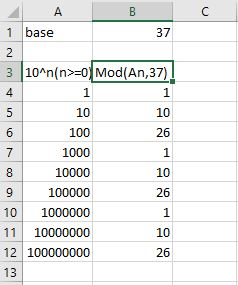
\includegraphics[width=2in]{images/divisibility_37}
}
\end{center}
\caption{Spreadsheet to compute the powers of 10 mod 37}
\label{powersOf10Mod37}
\end{figure}

Based on the results shown in Figure~\ref{powersOf10Mod37}, propose a divisibility rule to check whether numbers are divisible by 37. Apply your rule to the following numbers: 17094,   411108, 365412\\

\item Create a spreadsheet similar to the the spreadsheet in Figure~\ref{powersOf10Mod37}. Use your spreadsheet to find $\bmod(10^{n},111)$ for $0\leq n\leq 8$. Come up with a proposition for numbers in base $111$ and prove it similarly  the divisibility rule for numbers in base $11$ was proved in Proposition $~\ref{proposition:ModularArithmeticBases:divisibility by 11}$.
\end{enumerate}
\end{exercise}

Here's a number-magic trick involving divisibility that you can try on your friends. This example is thanks to Mr. Ogungbesan Adedoyinsola, a student at the University of Lagos.

\begin{example}{reverse9}
Let n=321. The digits in reverse order give $m=123$. Now subtract $n-m=321-123=198$. We can add the digits of $198$ to get $1+9+8=18$. Since the sum of the digits of $198$ is divisible by $9$, $198$ is divisible by $9$.
\end{example}

\begin{exercise}{}
Repeat Example~\ref{example:ModularArithmeticBases:reverse9} with the numbers: 4567, 314142, 583651.
\end{exercise}

Amazing!  But we have the mathematical tools to see why it works:

\begin{exercise}{decimal interger reverse order}
\begin{enumerate}[(a)]
\item Take any decimal integer, write the digits in reverse order, and subtract the reversed number from the original number. Show that the result is always divisible by $9$.\\
\item If the decimal integer has an odd number of digits, show that the result obtained in $(a)$ will always be divisible by $99$.
\item Show that if you take any decimal integer $n$, rearrange the digits, multiply by any power of 10, and  subtract $n$ from the resulting number, then your final result will always be divisible by 9. 
\end{enumerate}
\end{exercise}

There are many variations on this theme--maybe you can come up with one yourself.

\begin{exercise}{reverse even number digits}
Take any number with an even number of digits, reverse the number, and add the two together. Show that the result is always divisible by $11$.
\end{exercise}

\begin{exercise}{append reverse order}
Take any number with any number of digits. Write the digits in reverse order and append them to the end of the original number (for example, if the original number is 2834, the end result is the number 28344382). Show that the result is always divisible by $11$.(Hint: Think about Exercise~\ref{exercise:ModularArithmeticBases:reverse even number digits}). 
\end{exercise}

\begin{exercise}{}**
\begin{itemize}
\item
Factor the number 1001, and use your result to design a procedure that does the following.  Given a number $n$ with $m$ digits, using a single subtraction (and no multiplication)  construct a number $n'$ with $m-3$ digits such that $ \mod(n,7) = \mod(n',7), \mod(n,11) = \mod(n',11)$, and $\mod(n,13) = \mod(n',13)$.  
\item
Explain how it is possible to use your procedure to take an arbitrarily large number $n$ and obtain a number with three or fewer digits which has the same divisibility with respect to 7, 11, and 13 as $n$ does.
\item
Use your procedure to test (by hand)  the numbers 14142131356237 and 314159653589 for divisibility by 7,11, and 13, using only subtraction and 3 final divisiions of a 3-digit number.
\end{itemize}
\end{exercise}

\begin{exercise}{}**
\begin{itemize}
\item
Prove that the following rule works for divisibility by 7.  Given a $m$-digit number, remove the last digit $d_0$ to obtain a $m-1$-digit number, then subtract $2d_0$ from the $m-1$-digit number.  Then the new number has the same divisibility by 7 as the original number.
\item
Use the result in (a) to test the number 27182818284590 for divisibiilty by 7.
\item
Obtain similar rules for divisibility by 13 and 19.
\item Use your rules from (c) to test 27182818284590 for divisibility by 13 and 19.
\end{itemize}
\end{exercise}


\section{Decimal representations in other bases}
\label{sec:ModularArithmeticBases:DecimalRepresentationOtherBases}

We've mentioned above that we can express numbers in other bases besides base 10.  First we should explain what 
it means to represent a number in base $b$, where $b>2$ is a positive integer.  Recall that the base 10 number $d_n d_{n-1} \ldots d_1 d_0$ 
represents the integer:
\begin{equation*}
d_n d_{n-1} \ldots d_1 d_0 = d_n \cdot 10^n + d_{n-1}\cdot 10^{n-1} + \ldots + d_1 \cdot 10 + d_0.
\end{equation*}

For a number expressed in base $b$, we simply replace the 10's with $b$'s:

\begin{equation*}
(d_n d_{n-1} \ldots d_1 d_0)_b = d_n \cdot b^n + d_{n-1}\cdot b^{n-1} + \ldots + d_1 \cdot b + d_0.
\end{equation*}
 

For example, $(6342)_8$  represents the number:

\begin{equation*}
 (6342)_8 = 6 \cdot 8^3 + 3 \cdot 8^2 + 4 \cdot 8^1 + 2 \cdot 8^0.
\end{equation*}
 
 Note that if $(d_n d_{n-1} \ldots d_1 d_0)_b$ is a base $b$ representation, then all of the digits
 $d_0, \ldots d_n$ must be between 0 and $b-1$.

In order to be able to use other base representations effectively, we'll need to know how to convert numbers back and forth between 
other bases and base 10.  Let's see how this is done.

\begin{example}{137 base 6}
Find $137$ in base $6$.
I will solve this following the recursive method described in Section~\ref{sec:ModularArithmeticBases:DecimalRepresentationOtherBases},  but using base 6 instead of base 10. 
\begin{align*}
a_{0}&=137;~d_{0}=\bmod(137,6)=5 \\
a_{1}&=\frac{137-5}{6}=22;~d_{1}=\bmod(22,6)=4 \\
a_{2}&=\frac{22-4}{6}=3;~d_{2}=\bmod(3,6)=3 \\
a_{3}&=\frac{3-3}{6}=0
\end{align*}

Since $a_{3}=0$ we can stop. To write the solution take the moduli in reverse order. Therefore, $137$ in base $6$ is $345$.
\end{example}

\begin{example}{121 base 3}
Find $121$ in base $3$.  Once again using the recursive method

\begin{align*}
a_{0}&=121;\quad d_{0}=\bmod(121,3)=1 \\
a_{1}&=\frac{121-1}{3}=40;\quad d_{1}=\bmod(40,3)=1 \\
a_{2}&=\frac{40-1}{3}=13;\quad d_{2}=\bmod(13,3)=1 \\
a_{3}&=\frac{13-1}{3}=4;\quad d_{3}=\bmod(4,3)=1 \\
a_{4}&=\frac{4-1}{3}=1;\quad d_{4}\bmod(1,3)=1 \\
a_{5}&=\frac{1-1}{3}=0
\end{align*}

Since $a_{5}=0$ we do not have to continue. To write the solution take the moduli in reverse order. Therefore, $121$ in base $3$ is $11111$.
\end{example}


\begin{example}{65432 in base 3}
Find the 5th digit of $65432$ in base $3$. (This is the coefficient of $3^4$ in the base 3 representation). We may use 
Eq. \ref{eq:digit}, just replacing base 10 with base 3:

\begin{equation*}
d_{4}=\frac{\bmod(65432,3^{5})-\bmod(65432,3^{4})}{3^{4}}
\end{equation*}
\end{example}

You might be thinking that this is very similar to how we found the $k'th$ digit of a decimal integer in Section~\ref{decDigits} and you would be correct! The main difference  is that the base in the modulus is not a base of 10 but the base of the number we are finding (in the above example base 3). Also, instead of finding only one of the digits of a number in base 10, we are finding $\emph{all}$ the digits of a number in another base (in the above example it is base 3). We know we are done finding the entire number when $a_{n}=0$ and we write the final number in the reverse order of how we found the modulus'.

\begin{exercise}{numbers in other bases}
\begin{enumerate}[(a)]
\item Find $1567$ in base $5$.
\item Find $344$ in base $3$.
\item Find $7281$ in base $7$.
\item Find $3491$ base $4$.
\item Find $65432$ in base $3$.
\end{enumerate}
\end{exercise}
%% Answer:
%let $N=65432$.
%\begin{align*}
%a_{0}&=N=65432;~d_{0}=\bmod(N,3)=\bmod(65432,3)=2 \\
%a_{1}&=\frac{a_{0}-d_{0}}{3}=\frac{65432-2}{3}=21810;~d_{0}=\bmod(a_{1},3)=\bmod(21810,3)=0 \\
%a_{2}&=\frac{21810-0}{3}=727;~d_{2}=\bmod(723,3)=0 \\
%a_{3}&=\frac{723-0}{3}=241;~d_{3}=\bmod(241,3)=1 \\
%a_{4}&=\frac{241-1}{3}=80;~d_{4}=\bmod(80,3)=2\\
%a_{5}&=\frac{80-2}{3}=26,~d_{5}=\bmod(26,3)=2; a_{6}=\frac{26-2}{3}=8;~d_{6}=\bmod(8,3)=2\\
%a_{7}&=\frac{8-2}{3}=2,~d_{7}=\bmod(2,3)=2;~~a_{8}=\frac{2-2}{3}=0
%\end{align*}
%Since $a_{8}=0$ we can stop. The solution is all the $d_{k}$ values written in reverse order $(d_{7}d_{6}\dots d_{1}d_{0})$. Therefore, $N=65432$ in base $3$ is $n=22221002$. \\

Being able to represent numbers in base 2 is  important in computer science because this is how computers do arithmetic.  In base 2 the digits are called \term{bits}. All information that is stored in the computer is stored in the form of bits. A block of 8 bits is called a \term{byte}: computer memory is measured in terms of kilobytes, megabytes, or gigabytes. Integers are commonly stored as either 2 or 4 bytes.

\begin{example}{convert to base 2}
Find  $31$ in base $2$.
\begin{align*}
a_{0}&=31;~d_{0}=\bmod(31,2)=1;&a_{1}=\frac{31-1}{2}=15;~b_{1}=\bmod(15,2)=1\\
a_{2}&=\frac{15-1}{2}=15;~b_{2}=\bmod(14,2)=0;&a_{3}=\frac{14-0}{2}=15;~b_{3}=\bmod(7,2)=1\\
a_{4}&=\frac{7-1}{2}=15;~b_{4}=\bmod(6,2)=0;&a_{5}=\frac{6-0}{2}=15;~b_{5}=\bmod(3,2)=1\\
a_{6}&=\frac{3-1}{2}=15;~b_{6}=\bmod(1,2)=1;&a_{7}=\frac{1-1}{2}=0;~b_{7}=\bmod(0,2)=0
\end{align*}
Therefore $N=31$ written in base $2$ is $0110101$. If stored as a 2-byte integer, $N$ would be represented as $0b0000000000110101$  (the `0b' prefix indicates that the number is a binary number).
\end{example}
\begin{exercise}{numbers in base 2}
Express the following as 2-byte binary integers
\begin{enumerate}[(a)]
\item $73$
\item $235$
\item $1940$
\item $67037$
\end{enumerate} 
\end{exercise}

Base 16 is also often used: 
numbers in base 16 are called \term{hexadecimal} numbers.  In hexadecimal (or `hex') representation, the letters $A,B,C,D,E,F$ are used to represent $10, 11, 12, 13,14, 15$ respectively.
In many computer languages (like Java, C++, and Python), a hexadecimal number is indicated by the prefix `0x'.  So for example, the hex number $0xABCD$ signifies
$10\cdot 16^3 + 11 \cdot 16^2 + 12 \cdot 16^1 + 13$.

\begin{exercise}{hex}
Find the hex representations of the following decimal numbers
\begin{enumerate}[(a)]
\item $4095$
\item $10000$.
\item $123456$
\end{enumerate}
\end{exercise}

Converting numbers from base 10 to another base is fun! But how about converting numbers from another base to base 10? Piece of cake:

\begin{example}{121 base 3}
Convert $121$ in base $3$ to a number in base 10.\\

$(121)_{3}=1\cdot 3^{2}+2\cdot 3^{1}+1\cdot 3^{0}=1\cdot 9+2\cdot 3+1\cdot 1=(16)_{10}$
\end{example}

\begin{example}{4752 base 8}
Convert 4752 in base 8 to a number in base 10\\

$(4752)_{8}=4\cdot 8^{3}+7\cdot 8^{2}+5\cdot 8^{1}+2\cdot 8^{0}=4\cdot 512+7\cdot 64+5\cdot 8+2\cdot 1=(2538)_{10}$
\end{example}

Do you recognize this from before? All that we're doing is using the defining equation for base $b$ representation:

\begin{equation}
(n)_{b}=d_{m}\cdot (b)^{m}+d_{m-1}\cdot (b)^{m-1}+\hdots+d_{0}
\end{equation}

\begin{exercise}{numbers to base 10}
Convert the given numbers with their bases to a number in base 10:
\begin{enumerate}
\item 456 base 7
\item 32102 base 4
\item 8714 base 9
\end{enumerate}
\end{exercise}

Earlier we mentioned the importance of converting numbers in base 10 to base 2. It is just as important to convert numbers in base 2 to base 10.

\begin{example}{1011 base 2}
Convert 1011 in base 2 to a number in base 10.\\

$(1011)_{2}=1\cdot 2^{3}+0\cdot 2^{2}+1\cdot 2^{1}+1\cdot 2^{0}=1\cdot 8+0\cdot 4+1\cdot 2+1\cdot 1=(11)_{10}$
\end{example}

\begin{exercise}{base 2 to base 10}
Convert the given numbers in base 2 to a number in base 10:
\begin{enumerate}[(a)]
\item 10101
\item 11011001
\item 100111011
\end{enumerate}
\end{exercise}

\begin{exercise}{computerGraphics}
In computer graphics, colors are often represented using \term{RGB notation}. Colors have red, green, and blue components; and each component has an intensity level from 0 to 255, which can be stored as a single byte. Each byte is represented as two hex digits, so colors are represented as a six-digit hex number.  For example, 0xFFFFFF represents intensities of 255 for red, green and blue, corresponding to the color white, while 0x000000 represents black.  0xFF0000, 0x00FF00, 0x0000FF represent pure red, pure green, and pure blue respectively.

Find the red, green, and blue intensities for the following colors in hex representation:
\begin{enumerate}[(a)]
\item 0xAA45E2
\item 0x29A4F3
\item 0x774422
\end{enumerate}
\end{exercise}
 